\documentclass[../main.tex]{subfiles}
\begin{document}
\setchapterstyle{kao}
\setchapterpreamble[u]{\margintoc}
\setchapterimage[6.5cm]{images/twobrothers_cut.png}
\chapter[Two brothers: SU(2) and SO(3)]{Two brothers: SU(2) and SO(3)\footnotemark[0]}
\labch{Two-brothers}
\section{Motivation}
Why are we interested in SU(2) and SO(3)? First of all, because they are \textbf{physically relevant}. They appear in different context: 
\begin{marginfigure}[10mm]
    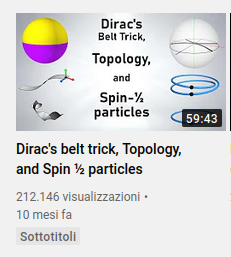
\includegraphics[]{images/videoSO(3).png}
    \caption[Video from YouTube]{For a more intuitive visualization of the topology of SO(3) and SU(2), we suggest \href{https://www.youtube.com/watch?v=ACZC_XEyg9U}{this video}. Pokémon evolution music starts at 15:28.}
\end{marginfigure}
\begin{itemize}
    \item the theory of angular momentum in QM is based on the projective unitary representation of SO(3), which at the end will be the true unitary representation of SU(2) (so it is a good reason to study both);
 \item $\textrm{U}(1)\otimes\textrm{SU}(2)$ appears as one of the ingredients in electroweak theory.
\end{itemize}
Moreover, it is paradigmatic: this phenomenon of brotherhood is actually universal. Another example we will encounter later is the relation between SL$(2,\mathbb{C})$ and the Lorentz group $\mathcal{L}$. We want to understand this phenomenon in the simplest possible example.

Brothers because they are very close related, but they are not the same group, despite the fact that they are sometimes confused in the literature. The reason why they are confused is because they share the same Lie algebra (the two Lie algebra are isomorphic). Now we want instead to emphasize the differences.
\section{Description of SO(3)}\index{SO(3)}
Context: we are in the three-dimensional euclidean space, which is $\mathbb{R}^3$ equipped with a scalar product:
\[
\mathbb{E}^3=\big(\mathbb{R}^3,(\dots{|}\dots)\big)
\]
where $(\dots{|}\dots)$ is a bilinear, symmetric and positive definite form. The orthogonal group, with respect to this structure, is defined as:
\[
\text{O(3)}=\Bqty{R\in\text{End}(\mathbb{R}^3):(Rv|Rw)=(v|w)\quad \forall\ v,w\in\mathbb{E}^3}
\]
As we have already said, this is equivalen to $R^TR=\mathbb{1}=RR^T$, hence by Binet's formula, this implies that {\color{red}$\text{det}R\in\{+1,-1\}$}. SO(3) is defined as:
\[
\text{SO}(3)=\{R\in\text{O(3)}:\text{det}R=1\}=\text{\underline{identity component of O$(3)$}}\marginnote{With the previous notation, it would have been O(3)$_0$ but that would have been ugly so people decided to call it SO(3).}
\]
As the determinant is a continuous function with only integer values, it must be constant on every connected component.

Our starting point is a little lemma:
\begin{lemma}[Every rotation is a rotation \textbf{around an axis}]
Let $R$ be an element of SO(3), then there exists $\hat{n}\in\mathbb{R}^3,||\hat{n}||=1$ such that:
\[
R\hat{n}=\hat{n} \qquad \text{(eigenvalue equation)}
\]
and that, in a suitable ortho-normal basis $\{\hat{n},\hat{a},\hat{b}\}\subseteq\mathbb{R}^3$:
\[
R\xleftrightarrow[]{}{}\left(\begin{array}{c:cc}
    1 & 0 & 0 \\
    \hdashline
    0 & \cos\phi & \sin\phi \\
    0 & -\sin\phi & \cos\phi
\end{array}
\right)\quad \text{for some }\,\phi\in[0,\pi]
\]
If $\phi\not\in\{0,\pi\}$ then in the description above $(\hat{n},\phi)$ is unique.
\end{lemma}
This might seem tautological but it is not! Suppose we have a rotation around this axis and we compose it with a rotation around this other axis: it is not obvious that the composition of the two is still a rotation around an axis. Instead this is true and this is what we are going to prove.
\begin{proof}\marginnote[-65 mm]{\textbf{Teorema:}
Sia $T:V\to V$ un endomorfismo di uno spazio vettoriale $V$ sul campo $\mathbb{K}$. Fissiamo una base $\pazocal{B}=\left\{v_1,\dots,v_n\right\}$ di  $V$, e sia $A\in M_{n,n}(\mathbb{K})$ la matrice che rappresenta $T$ rispetto a $\pazocal{B}$. Allora si ha:
\begin{enumerate}
    \item la funzione $p_T:\mathbb{K}\to\mathbb{K}$ data da \(p_T(\lambda)=\det\left(A-\lambda I_n\right)\) non dipende dalla base $\pazocal{B}$ scelta;
    \item $p_T$ è un polinomio di grado $n$ in cui il coefficiente direttivo è $(-1)^n$, il termine noto è $\det A$ e il coefficiente di $\lambda^{n-1}$ è $(-1)^{n-i}\tr A$, dove la traccia $\tr A$ della matrice $A$ è la somma degli elementi sulla diagonale;
    \item $\lambda_0\in \mathbb{K}$ è un autovalore di $T$ se e solo se $p_T(\lambda_0)=0$.
\end{enumerate}}
\circled{1} We prove that $R$ admits the \textbf{eigenvalue} 1. The eigenvalues are the zeroes of the \textbf{characteristic polynomial} \sidecite{abate2006geometria}: 
\[
\begin{WithArrows}\WithArrowsOptions{displaystyle}
\chi(\lambda)
&=\text{det}(\lambda\mathbb{1}-R)=\Arrow{see sidenote}\\
&=\lambda^3-c_2(R)\lambda^2+c_1(R)\lambda-\text{det}R=\Arrow{see sidenote}\\
&=\lambda^3-\text{tr}(R)\lambda^2+c_1(R)\lambda\;{\color{red}-1}
\end{WithArrows}
\]
Therefore $\exists\;\lambda_0\in\mathbb{R}_+$ eigenvalue of $R$ (\reffig{char_polynomial}). We also know its value, suppose that $\lambda_0$ solves the eigenvalue equation $Ru=\lambda_0u$.
\[
(Ru|Ru)=(u|u)=\lambda_0^2(u|u)\quad \Rightarrow\lambda_0^2=1,\lambda_0=1
\]
We define the versor to be $u$ normalized: $\hat{n}:=\frac{u}{||u||}$ so that $R\hat{n}=\hat{n}.$
\begin{marginfigure}[-30mm]
    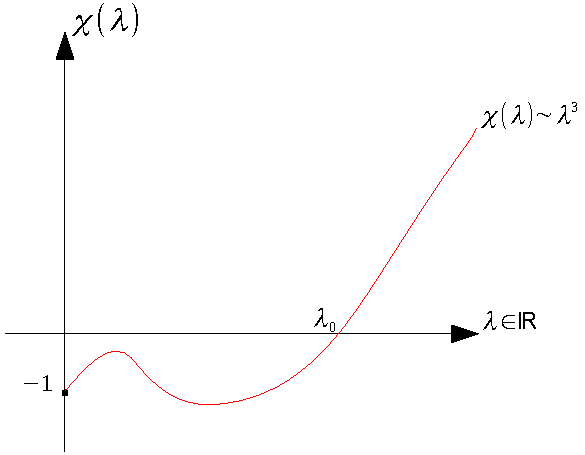
\includegraphics[width=1\linewidth]{images/char_poly.pdf}
	\caption[The characteristic polynomial as a function of real $\lambda$.]{The characteristic polynomial as a function of real $\lambda$. Since it has to go from $-1$ to $+\infty$, it has to pass through zero at some point.}
	\labfig{char_polynomial}
\end{marginfigure}
\circled{2} $R\in\text{End}(\mathbb{R}^3)\subseteq\text{End}(\mathbb{C}^3)$. $\lambda_0=1$ and, as $\text{det}R=1$, $\lambda_1\lambda_2=1$ in the form $e^{i\phi}$ and $e^{-i\phi}$ for $\phi\in[0,\pi]$. Excluding $\phi\in\{0,\pi\}$, we set the \textbf{eigenvalue equation in} $\mathbb{C}^3$:
\[
\begin{cases}
Rz=e^{i\phi}z \qquad &z=a+ib\in\mathbb{C}^3 \\    
Rz^*=e^{-i\phi}z^* \qquad & z=a-ib\in\mathbb{C}^3 
\end{cases}
\]
We now compute:
\begin{align*}
Ra&=R\left[\frac{1}{2}(z+z^*)\right]=\frac{1}{2}(Rz+Rz^*)=\frac{e^{i\phi}z+e^{-i\phi}z^*}{2}=\frac{e^{i\phi}+e^{-i\phi}}{2}a+i\frac{e^{i\phi}-e^{-i\phi}}{2}b=a\cos\phi-b\sin\phi\\
Rb&=R\left[\frac{1}{2i}(z-z^*)\right]=\frac{1}{2i}(Rz-Rz^*)=\frac{e^{i\phi}z-e^{-i\phi}z^*}{2i}=\frac{e^{i\phi}-e^{-i\phi}}{2i}a+\frac{e^{i\phi}+e^{-i\phi}}{2}b=a\sin\phi+b\cos\phi
\end{align*}
In the basis $\{\hat{n},\hat{a},\hat{b}\}$, we have:
\[
R\xleftrightarrow[]{}{}\left(\begin{array}{c:cc}
    1 & 0 & 0 \\
    \hdashline
    0 & \cos\phi & \sin\phi \\
    0 & -\sin\phi & \cos\phi
\end{array}
\right)
\]
It is left as an exercise to check that $\{\hat{n},\hat{a},\hat{b}\}$ are \textbf{orthogonal.}\marginnote{It is also left as an exercise the two extreme cases $0$ and $\pi$.}
\end{proof}
\subsection{Parametric description of SO(3)}
The idea is to take an element of $R\in\textrm{SO}(3)$ and to associate the pair $(\hat{n},\phi)$. We have seen that the pair is unique (except at the extreme cases $\phi=0$ and $\phi=\pi$), so we could have the idea to condensate the information of the pair in a single vector, multiplying the $\phi\hat{n}$.\marginnote{The bar  over the $\mathbb{B}$ means that the ball is closed.} This is of course a vector in $\mathbb{R}^3$, but it is also a vector in the three dimensional ball of radius $\pi$. Therefore we can write
\begin{align*}
\text{SO(3)}&\xrightarrow[]{}\frac{\bar{\mathbb{B}}^3(0,\pi)}{\sim_{\text{antip}}}\\
R&\mapsto\phi\hat{n}\in\mathbb{R}^3
\end{align*}
where $\bar{\mathbb{B}}^d(x_0,R)=\{x\in\mathbb{R}^d:|x-x_0|\le R\}$. Each point of the ball corresponds to a rotation. If we do not include the $\sim_{\text{antip}}$ relation, this map would not be well defined, because to every rotation corresponds a pair $(\phi, n)$, but with a \textit{caveat} that appears at the boundary: the description is not faithful unless we identify the opposite points on the surface. Therefore, for two points on the surface $p,\tilde{p}\in\partial\mathbb{B}^3(0,\pi)$ we say that {\color{red}$p\sim_{\text{antip}}\tilde{p}$} if $\tilde{p}=-p$. Basically we must identify antipodal points on the boundary of the ball because they correspond to the \textbf{same rotation}.
\begin{marginfigure}[-40mm]
    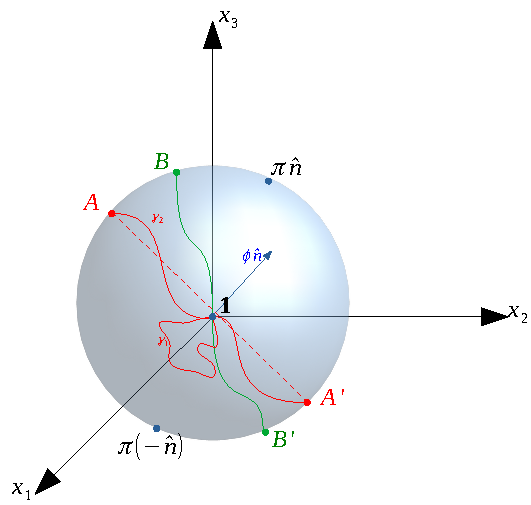
\includegraphics[width=1\linewidth]{images/equivalence.pdf}
	\caption[Parametric description of $\textrm{SO}(3)$]{Parametric description of $\textrm{SO}(3)$.} %MANCANO DETTAGLI GRAFICO}
	\labfig{equivalence}
\end{marginfigure} %Incomplete figure
\underline{\textbf{Fact:}} In SO(3) there are two \textbf{inequivalent classes of continuous paths:}
\begin{itemize}
    \item those which can be continuously deformed to $\mathbb{1}$;
    \item those which cannot, namely those ones passing through $\partial\mathbb{B}^3$, because the two points on the boundary are actually the \textbf{same point}. If we want to deform these paths, we have to bring the points next to each other but this is not possible since they always have to remain \textbf{antipodal}.
\end{itemize}
Therefore, \textbf{SO(3) is \underline{not} simply connected.}
\section{Description of SU(2)}
\begin{lemma}
$\forall\alpha,\beta\in\mathbb{C}$ with $|\alpha|^2+|\beta|^2=1$, one has that:
\begin{equation}\labeq{matrixSU2}
M=\begin{pNiceArray}{cc}[margin]
\alpha & -\overline{\beta} \\
\beta & \overline{\alpha}
\end{pNiceArray}
\quad (\star)
\end{equation}
is in SU(2). Moreover, \textbf{every} $M\in\textrm{SU}(2)$ can be written in the form (\ref{eq:matrixSU2}) for a \textbf{\underline{unique} pair $(\alpha,\beta)\in\mathbb{C}^2$ satisfying the constraint stated above}.
\end{lemma}
\begin{proof}
The proof is left as an exercise for the reader.
\end{proof}
This means that:\marginnote{With "dimension", we always mean \textit{real} dimension; so $\dim{\mathbb{C}^2}=4$} 
\[
\textrm{SU}(2)\approx\{(\alpha,\beta)\in\mathbb{C}^2:|\alpha|^2+|\beta|^2=1\}=S^3=\{x\in\mathbb{R}^4:|x|=1\}
\]
(at least as a set, or better, as a topological space). The description is a map:
\begin{align*}
\text{SU(2)}&\twoheadrightarrow S^3\marginnote{The double head on the arrow means that it is surjective.}\\
M&\mapsto(\alpha,\beta)
\end{align*}
Notice that:
\[
\begin{cases}
+\mathbb{1}&\mapsto(+1,0)\\
-\mathbb{1}&\mapsto(-1,0)
\end{cases} 
\]
are two antipodal points. This map is surjective (every pair $\alpha,\beta$ on the sphere defines an element of $\textrm{SU}(2)$) and injective (because these two parameters are unique). One checks that $\varphi$ and $\varphi^{-1}$ are \textbf{continuous} (so it is really a topological identification). How can we visualize $S^3$? Let us start with dimension two as in \reffig{visualization}, taking the two dimensional ball of centre zero and radius one.
\begin{figure*}[h]
    \centering
    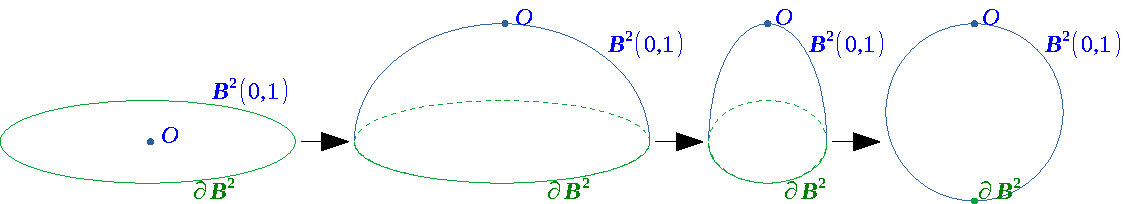
\includegraphics{images/visualization.pdf}
    \caption{Continuous deformation of $S^2$.}
    \labfig{visualization}
\end{figure*}

\underline{$d=2$}: We start bending, with a continuous deformation, the disk in such a way that the boundary $\partial\mathbb{B}^2$ is collapsed to a point (the South pole); in the end we will have that our disk has became a two-sphere, where all the boundary of the two-dimensional disk is now collapsed to a point: it is a quotient \[
S^2\approx\frac{\mathbb{B}^2}{\partial\mathbb{B}^2}
\]
Notice also that if we start from the disk, we have two distinguish points:
\begin{itemize}
    \item zero (the centre of the disk) which becomes the North Pole;
    \item the boundary (which will become a point) which becomes the South Pole.
\end{itemize}
\underline{$d=3$}: By the exact same argument, we obtain that: 
\[
S^3\approx\frac{\mathbb{B}^3}{\partial\mathbb{B}^3}
\]
And in this case $\textrm{SU}(2)$\textbf{ is simply connected}. 
\section{Comparison of the brothers}
SO(3) is the three-dimensional ball (center in the identity, radius $\pi$ if you want to make it metrically, but topologically is just a ball) divided by the relation of antipodal equivalence but only on the surface: $A$ is equivalent to $A'$, $B$ is equivalent to $B'$, as shown in \reffig{equivalence}. SO(3)$\approx\mathbb{B}^3\slash\sim_{\textrm{antip}}$

On the other hand, we have SU(2) which is still a three-dimensional ball but divided by the relation that all the boundary of the ball is a unique point: SU(2)$\approx\mathbb{B}^3\slash\partial\mathbb{B}^3$. Is SU(2) simply connected? Yes! They look very much the same in the neighbourhood of the identity, actually we will see that they have the same Lie algebra, but not globally: if we move far away from the center of the ball and reach the boundary we see that there are differences in the two cases. 
\subsubsection{Brotherhood: $\textrm{SU}(2)$ is a 2-covering of $\textrm{SO}(3)$}
We are going to prove the following theorem:
\begin{theorem}\labthm{lie-group2-to-1}
We exhibit a Lie group homomorphism:
\[
    \phi : \textrm{SU}(2) \twoheadrightarrow \textrm{SO}(3)
\]
which is \textbf{surjective} and is \textbf{2-to-1}, i.e. $\forall \ R \in \textrm{SO}(3)$ if we take the set which consists only of these points and we take the pre-image via $\phi$, the number of elements is
\[
\abs{\phi^{-1}\Bqty{R}}=2
\]
\end{theorem}
\underline{\textbf{Visualization:}} this statement is in every book, but what it is not present is how to visualize that.
\begin{figure}[h!]
    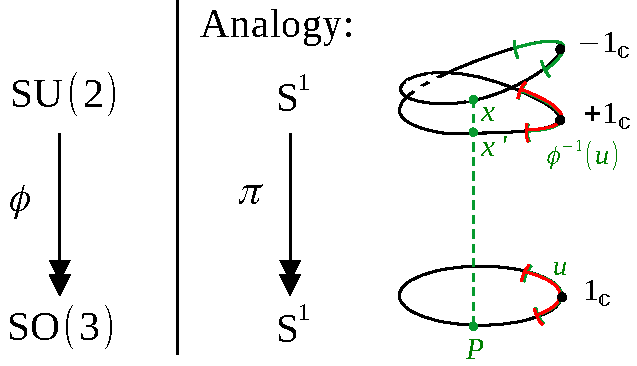
\includegraphics[width=1\linewidth]{images/analogy_SU2_SO3.pdf}
	\caption[Visual analogy of $\textrm{SU}(2)$ as a 2-covering of $\textrm{SO}(3)$]{Visual analogy of $\textrm{SU}(2)$ as a 2-covering of $\textrm{SO}(3)$. On the right hand side there is the simplest possible example of 2 fold covering (except the real line, but it is topologically trivial). It says that if we take a neighborhood $u$ of neutral element in the arrival space, the pre-image contains two pieces. By selecting of of the two (the red one), it is completely identified with a neighborhood of the identity in the starting space by a diffeomorphism which also locally preserves the product (it can be checked).}
	\labfig{analogy-su2-so3}
\end{figure}

The good way to write that is to write it vertically. If we write $\textrm{SU}(2)$ above and $\textrm{SO(3)}$ below as in \reffig{analogy-su2-so3}, this is the analogous of covering twice the circle with the circle. We know we can identify the circle with the set of unimodular complex numbers
\[
S^1\equiv \textrm{U}(1)=\Bqty{z\in \mathbb{C}: \ \abs{z}=1}
\]
And we can think of a very simple map $\pi$ such that:
\[
\begin{split}
    \pi : S^1 &\xrightarrow[]{\textrm{hom}} S^1\\
    z &\mapsto z^2
\end{split}
\quad \textrm{in fact: } \left(zw\right)=z^2w^2 \ \Rightarrow \ \text{\parbox{3 cm}{\centering Homomorphism of \\[-4pt] Lie groups\\[-4pt] surjective, 2-to-1}}
\]
The map is surjective and it is an homomorphism of groups and we can also check it is smooth, so it is an homomorphism of Lie groups. This case can be visualized very well; for the pre-image we try to make another circle in such a way that every point of the other circle fits exactly on the vertical line to that of its image. With the eyes of our imagination we can think a similar picture in which the three dimensional ball, with all the boundary identified, covers twice the three dimensional ball with antipodal points in the boundary identified (for the lack of dimensions we live in, unfortunately we are not able to draw that).

From \sidecite{Hall2015}. Consider the linear space of all the $2\times 2$ matrices such that:
\begin{equation}\labeq{spaceV-ad-traceless}
V=\Bqty{X\in\textrm{Mat}(2,\mathbb{C}): \ X^\ast=X, \tr(X)=0}
\end{equation}
It is obvious that it is a linear space, we just check that elements $X\in V$ can be written by using three independent real parameters. First of all the matrix should be self-adjoint (elements on the diagonal are real) in such a way that the trace is zero
\[
X=
\begin{pmatrix}
x_1 & x_2+ix_3\\
x_2-ix_3 & -x_1
\end{pmatrix} \quad \textrm{for } x_1,x_2,x_3\in \mathbb{R}
\]
Hence $V\underset{\textrm{Linear}}{\cong} \mathbb{R}^3$. 
\begin{kaobox}
To the professor's taste, it would be more elegant to decompose in another way, using Pauli's matrices\marginnote{From \href{https://en.wikipedia.org/wiki/Pauli_matrices}{Wikipedia}: In meccanica quantistica le \textbf{matrici di Pauli} sono un insieme di matrici $2\times 2$ complesse, hermitiane e unitarie. Usualmente indicate dalla lettera greca $\sigma$ (\textit{sigma}). Devono il loro nome al fisico Wolfgang Pauli e sono così definite:
\[
\begin{split}
    \sigma_1 \equiv \sigma_x &\equiv \begin{pmatrix} 0 & 1 \\ 1 & 0 \end{pmatrix}\\
    \sigma_2 \equiv \sigma_y &\equiv \begin{pmatrix} 0 & -i \\ i & 0 \end{pmatrix}\\
    \sigma_3 \equiv \sigma_z &\equiv \begin{pmatrix} 1 & 0 \\ 0 & {-1}
\end{pmatrix}
\end{split}
\]
}. This would give a slightly different but completely equivalent representation
\[
X=\sum_{j=1}^3x_j\sigma_j=x_1\sigma_1+x_2\sigma_2+x_3\sigma_3=
\begin{pmatrix}
x_3 & x_1-ix_2\\
x_1+ix_2 & -x_3
\end{pmatrix}
\]
but he prefers to adhere to \cite{Hall2015} to not get confused.
\end{kaobox}
Then for $X,Y\in V$ one has (it can be computed)
\begin{equation}\labeq{scal-prod-iso-r3}
{\color{red}\left(X|Y\right)_{V}:=}\,\frac{1}{2}\tr\pqty{X^\ast Y}=\sum_{j=1}^3x_jy_j=\left(x|y\right)_{\mathbb{R}^3}
\end{equation}
On the r.h.s. we have a scalar product and so we can use it to have for free a scalar product between $X$ and $Y$ (the red part); then, since we have a linear isomorphism and identification of scalar products, it means that our space $V$ equipped with this scalar product of matrices $\left(V,(\dots|\dots)_V\right)$ is identified with the three-dimensional euclidean space\index{three-dimensional euclidean space} $\mathbb{E}^3$, that is how we call $\mathbb{R}^3$ equipped with the ordinary scalar product.

So $V$ is just a rather strange way to represent $\mathbb{R}^3$ with the scalar product defined in \refeq{scal-prod-iso-r3}. We do this strange representation, because once we represent $\mathbb{R}^3$ as two-by-two matrices, then we can act on them with two-by-two unitaries. Indeed, we cannot take two-by-two unitaries and let it act on three-component vectors, we should invent a representation, that is exactly what we are doing. So, first we identify $\mathbb{R}^3$ with a special space of two-by-two matrices (self adjointed and traceless), and then we let the unitary act on this space.
\begin{lemma}
\lablemma{phiuxu}
For each $U\in\textrm{SU}(2)$ define an action of $U$ on the linear space $V$ defined in \refeq{spaceV-ad-traceless}, by the following formula:
\[
\phi_U(X)=UXU^{-1}
\]
Then $\phi_U$ maps $V$ into $V$ and preserves the scalar product in $V$
\end{lemma}
\begin{corollary}
Hence $\phi_U:\; V\to V$ can be identified with an element of $\textrm{O}(V)\cong \textrm{O}(3)$.
\end{corollary}
\begin{proof}
We prove the Lemma, the corollary is obvious.
\renewcommand{\labelenumi}{\Alph{enumi})}
\renewcommand{\labelenumii}{\Alph{enumi}\arabic{enumii})}
\begin{enumerate}
    \item We have to check that $\phi_U(X)\overset{?}{\in}V$ for $X\in V$. This means that we have to check two things:
    \begin{enumerate}
        \item That $\phi_U(X)$ is self-adjoint. To do that we compute the adjoint\marginnote{Since the adjoint is an anti-homomorphism it inverts the order}
        \[
        \phi_U(X)^\ast=\pqty{UXU^{-1}}^\ast\overset{\mathclap{\tikz \node {$\downarrow$} node [above=1.25ex] {\footnotesize The adj. is anti-homo + $U$ is unitary};}}{=}\left(U^\ast\right)^\ast X^\ast U^\ast\underset{\mathclap{\tikz \node {$\uparrow$} node [below=1ex] {\footnotesize $X$ is self-adj. and $U$ is unitary};}}{=}UXU^{-1}=\phi_U(X) \quad \checkmark
        \]
        \item That it is traceless. There are two arguments we can use: either the fact that the trace is cyclic or use the fact that the trace is invariant by unitary equivalence; in both cases:
        \[
        \tr\left(\phi_U(X)\right)=\tr\left(UXU^{-1}\right)\underset{\mathclap{\tikz \node {$\uparrow$} node [below=1ex] {\footnotesize One of the two arguments};}}{=}\tr(X) \quad \checkmark
        \]
    \end{enumerate}
    \item We have to check that $\phi_U$ preserves the scalar product. For $X,Y\in V$ let us try to compute:
    \[
    \begin{WithArrows}\WithArrowsOptions{displaystyle}
    \left(\phi_U(X)\;|\;\phi_U(Y)\right)_V\overset{(\ref{eq:scal-prod-iso-r3})}{=}\frac{1}{2}\tr\left(UXU^{-1}\cdot UYU^{-1}\right)
    &=\frac{1}{2}\tr\left(UXYU^{-1}\right)\Arrow{Cyclicality of the trace}\\
    &=\frac{1}{2}\tr\left(XY\right)\\
    &=\left(X\:|\;Y\right)_V \quad \checkmark
    \end{WithArrows}
    \]
\end{enumerate}
\end{proof}
Basically $\phi_U$ identifies two-by-two unitaries to each isometries of three-dimensional euclidean space, so with orthogonal endomorphisms. Are there rotations? How do we know that they are in $\textrm{SO}(3)$? But before, let us check that it is a homomorphism.
\begin{lemma}
For every $U,W\in\textrm{SU}(2)$ one has
\[
\phi_{UW}=\phi_U\circ\phi_W
\]\marginnote{At the end it will be $\textrm{SO}(3)$ instead of $\textrm{O}(3)$.}
Moreover $\phi:\textrm{SU}(2)\to\textrm{O}(3)$ is $C^\infty$-smooth. Hence $\phi$ \textbf{is a Lie group homomorphism}.
\end{lemma}
\begin{proof}
It is splitted in two parts, the first one is the algebraic one: we compute on a generic $X$
\[
\begin{WithArrows}\WithArrowsOptions{displaystyle}
\phi_{UW}(X)&=\left(UW\right)X\left(UW\right)^{-1}\Arrow{The composition is associative + \\ inversion echange the order}\\
&=UWXW^{-1}U^{-1}\Arrow{Put the {\color{ForestGreen}brackets} wherever we want}\\
&=U{\color{ForestGreen}(}WXW^{-1}{\color{ForestGreen})}U^{-1}=\\
&=\phi_U\left(\phi_W(X)\right)=\\
&=\phi_U\circ\phi_W(X)
\end{WithArrows}
\]
As for $C^\infty$-smoothness, we will not do it in detail, but we can make the following reasoning, take
\[
\phi_U(X)=UXU^{-1}
\]
and suppose we start with $U=U_0$, a point in $\textrm{SU}(2)$ and then to vary smoothly, what happens? Well, $U^{-1}$ depends smoothly on $U$, because the inversion is smooth (as it happens in every Lie group), the composition is smooth, then ($X$ is fixed) $XU^{-1}$ is also smooth. Then we apply again $U$ on the other side and we get something smooth. If we want to be more formal, we could say that
\[
\begin{split}
G\times G &\to G\\
U\underset{\mathclap{\tikz \node {$\uparrow$} node [below=1ex] {\footnotesize \text{\parbox{3 cm}{\centering Inversion \\[-4.2pt] is smooth}}};}}{\overset{{\color{red}C^\infty}}{\mapsto}}\left(U,U^{-1}\right)\underset{\mathclap{\tikz \node {$\uparrow$} node [below=1ex] {\footnotesize \text{\parbox{3 cm}{\centering Composition \\[-4.2pt] is smooth}}};}}{\overset{{\color{red}C^\infty}}{\mapsto}}\left(U,XU^{-1}\right)&\underset{\mathclap{\tikz \node {$\uparrow$} node [below=1ex] {\footnotesize \text{\parbox{3 cm}{\centering Composition is\\[-4.2pt] \textbf{jointly smooth}}}};}}{\mapsto} UXU^{-1}
\end{split}
\]
\end{proof}
At the moment the arrival space is $\textrm{O}(3)$, but now we do the following reasoning: since the map $\phi$ is smooth, it is also continuous; but a continuous map maps a connected set into a connected set. $\textrm{SU}(2)$ is connected\sidenote{is a three-dimensional sphere}, then a continuous map should bring $\textrm{SU}(2)$ into a connected component of $\textrm{O}(3)$. Since the identity goes into the identities\sidenote{Every homomorphism must preserve the neutral element} then the whole $\textrm{SU}(2)$ goes to the identity component of $\textrm{O}(3)$, which is $\textrm{SO}(3)$. It is an abstract, but very clear, argument which uses only continuity and connectedness. Let us write it:
\begin{itemize}
    \item Since $\phi$ is smooth, it is continuos, then it maps \textbf{connected sets} in \textbf{connected sets}.
    \item As $\textrm{SU}(2)\simeq S^3$ is connected, its image via $\phi$, namely $\phi\left(\textrm{SU}(2)\right)$ is connected, hence it is contained in a connected component of $\textrm{O}(3)$.
    \item But we know\sidenote{since $\phi$ is an homomorphism} that $\phi\left(\mathbb{1}_{\textrm{SU}(2)}\right)=\mathbb{1}_{\textrm{O}(3)}$.
    \item Hence, we conclude that:
    \[
    {\color{red}\phi\left(\textrm{SU}(2)\right)\subseteq\textrm{SO(3)}}
    \]
\end{itemize}
\begin{exercise}
Is $\phi$ surjective to $\textrm{SO}(3)$? Yes (exercise)
\end{exercise}
\underline{Is $\phi$ injective?} No, indeed one sees 
\[
\phi_{\mathbb{1}}(X)=X=\phi_{-\mathbb{1}}(X)
\]
So both identity and minus the identity of $\textrm{SU}(2)$ are mapped into the identity of $\textrm{SO}(3)$. Now we claim that the same happens for every point in $\textrm{SO}(3)$ which has exactly two pre-images. We can prove that in one line: since $\phi$ is a continuous map, the number of pre-images is locally constant, therefore it is constant in every connected component. But $\textrm{SO}(3)$ (the rotations) is a connected space, then it is constant everywhere. At the identity we checked\sidenote{Actually it can be checked that there are no other pre-images} that the number of preimages is two, then it is done.

\textit{The number of preimages (called \textbf{cardinality}\index{Cardinality)} $\abs{\phi^{-1}\Bqty{P}}$) is \textbf{locally constant as $\phi$ is smooth}. Hence it is constant on every connected component. But $\textrm{SO}(3)$ is connected, hence:
\[
\abs{\phi^{-1}\Bqty{P}}\underset{\forall P}{=}\abs{\phi^{-1}\Bqty{\mathbb{1}_{\textrm{SO}(3)}}}=2
\]}
Let us emphasize the beauty of this kind of topologically arguments, they do not require computations.\marginnote{The same can be proved by doing a lot of computations: taking a rotation, computing how many pre-images there are and one would get exactly the same result after half an hour.} Putting all the pieces together, we have proved the \vrefthm{lie-group2-to-1}.
\end{document}
% 41 min